\documentclass[a4paper, 12pt]{article}

\usepackage[english]{babel}
\usepackage[utf8]{inputenc}
\usepackage{amsmath}
\usepackage{indentfirst}
\usepackage{graphicx}
\usepackage[colorinlistoftodos]{todonotes}
\usepackage{natbib}
\usepackage{xcolor}


\begin{document}

\begin{titlepage}
	\begin{center}

\vspace{10pt}
\begin{figure}[!ht]
\centering

\includegraphics[scale=0.2]{img/logo_university.png}
\end{figure}


\huge{Universidade Federal de Pernambuco}
\huge{Centro de Informática}

        
        \vspace{85pt}
        
		\textbf{\LARGE{Machine Learning for Hand Gesture Recognition Applied to LIBRAS (Brazilian Sign Language)}}\\
		\vspace{35pt}
		\large{Discipline: Introduction to Computing - IF668\cite{course}}
		\vspace{80pt}
		
	\end{center}
	
	\begin{flushleft}
		\begin{tabbing}
			Students\qquad\qquad\= Eric Vinícius de Lima\cite{eric}\\
			\>Michel Leonidas Aleixo da Silva\cite{michel}\\
			Professor\> Adriano Lorena Inacio de Oliveira\cite{adriano} \\
			Time\> Tuesday - 10:00-12:00 AM\\
		
	\end{tabbing}
		  
	\end{flushleft}
	
	\begin{center}
		\vspace{25pt}
		Recife, October 24, 2021
	\end{center}
\end{titlepage}

%%%%%%%%%%%%%%%%%%%%%%%%%%%%%%%%%%%%%%%%%%%%%%%%%%%%%%%%%%%
\newpage
\tableofcontents
\thispagestyle{empty}

\newpage
\pagenumbering{arabic}

%%%%%%%%%%%%%%%%%%%%%%%%%%%%%%%%%%%%%%%%%%%%%%%%%%%%%%%%%
%%%%%%%%%%%%%%%%%%%%%%%%%%%%%%%%%%%%%%%%%%%%%%%%%%%%
\section{Introduction}

After an introductory class on Machine Learning given by Professor Adriano L. I. Oliveira, a project was requested with the general objective of applying this knowledge of Artificial Intelligence in practice. Building a program that involved machine learning with models based on Text, Images, Numbers or Sounds, applicable to any real or non-real situation.

The Brazilian Sign Language - LIBRAS - is considered official in the country since 2005\cite{planalto}, but even with more than 9 million hearing impaired people (2010)\cite{ibge}, it is still not taught in public schools, making this language learning even more difficult and, consequently, the communication with a hearing impaired.

With that, we decided to develop an application that uses Machine Learning capable of judging with precision if the gesture made with the hand is or not a vowel of the Brazilian Sign Language, through a webcam.

\begin{figure}[!ht]
\centering
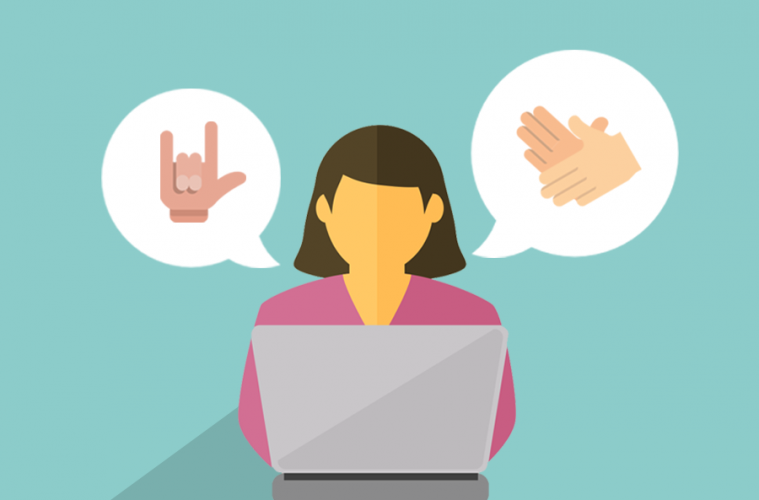
\includegraphics[scale=0.2]{img/inclusion.png}
\caption{Inclusion and accessibility of hearing impaired\cite{figure_1}}
\label{figure_1}
\end{figure}


%%%%%%%%%%%%%%%%%%%%%%%%%%%%%%%%%%%%%%%%%%%%%%%%%%%%%%%%%%%%%%%
\section{Tools Used}

For this experiment, the programming language Python\cite{python} was used together with the Mediapipe\cite{mediapipe} and OpenCV\cite{opencv} frameworks, in addition to the Machine Learning for Kids\cite{ml4kids} platform for processing the results with the Watson Assistant from IBM\cite{watson}.

\begin{figure}[!ht]
\centering
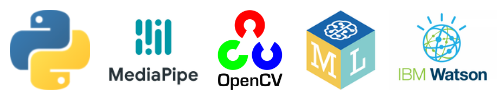
\includegraphics[scale=0.9]{img/tools.png}
\caption{Tools used in this project}
\label{figure_2}
\end{figure}

%%%%%%%%%%%%%%%%%%%%%%%%%%%%%%%%%%%%%%%%%%%%%%%%%%%%%%%%%%%%%%

\section{Experimental Procedure}

Initially, it was studied how the recognition of a hand by the computer works. We can usually represent it computationally as a 21-vertex graph. To reduce complexity, we decided to work with just 11 of them.
 
\begin{figure}[!ht]
\centering
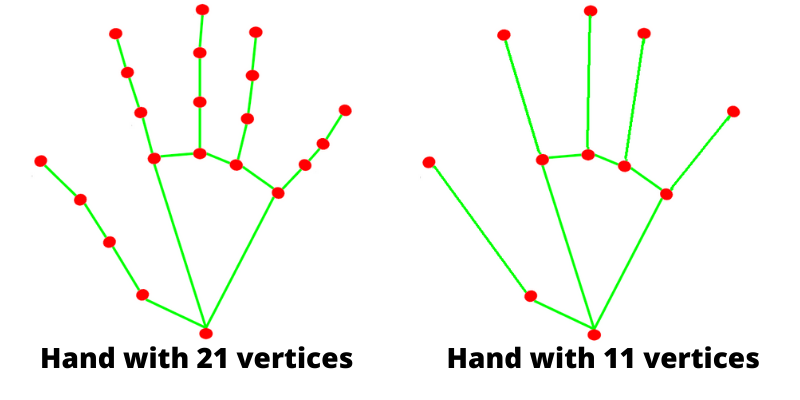
\includegraphics[scale=0.4]{img/hand_vertices.png}
\caption{Hand with different amount of vertices}
\label{figure_3}
\end{figure}

Also, it was decided to judge only the vowels and not the entire alphabet in LIBRAS. Machine Learning for Kids allows only 10 labels to work with numbers. Each vertex has a coordinate containing 2 values: x and y axis. An impediment was then introduced, so it was decided to further reduce the number of vertices, now to just 5. The most relevant vertices were then chosen, following the following gestures:
 
 
 \begin{figure}[!ht]
\centering
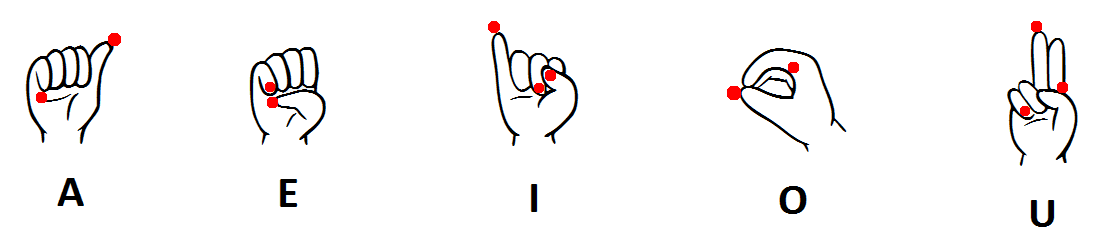
\includegraphics[scale=0.3]{img/hands_gestures.png}
\caption{Vowels in LIBRAS with main vertices}
\label{figure_4}
\end{figure}
 
Following the vertex naming adopted by Mediapipe, the chosen vertices were: 0-wrist, 4-thumb-tip, 5-index-finger-mcp, 12-middle-finger-tip and 20-pinky-tip. With that, the elaboration of the project code was started, and it was divided into 3 parts:


\newpage
\subsection{Data Collect:}
This first part of the project was to use the mentioned libraries to collect the data and treat. The OpenCV was then used to recognize a camera and perform some image settings. Then, we use some solutions present in Mediapipe, to detect and recognize hands, in addition to printing them on the screen. MediaPipe treats the hand with 21 vertices, so we treat these vertices to only take 5 of them and eject the z-axis as it is not needed for the project.

Finally, it was possible to collect, through keys pressed on the keyboard, the x and y axes of each of the chosen vertices.

 \begin{figure}[!ht]
\centering
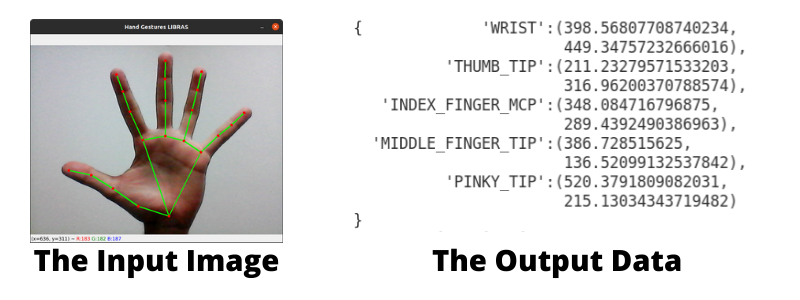
\includegraphics[scale=0.5]{img/data_collect.png}
\caption{Collecting Data}
\label{figure_5}
\end{figure}



\subsection{Populate Training Database:}
To communicate with Machine Learning for Kids, we use its API, in which it is possible to request the classification of data and also request the filling of the training database, and integrate it into the project through the Python Request library\cite{requests}. For this, another module responsible for making this communication, was created in addition to generating an API access key directly in Machine Learning for Kids, as well as performing other configurations, such as creating labels for the vowels that will be filled.

 \begin{figure}[!ht]
\centering
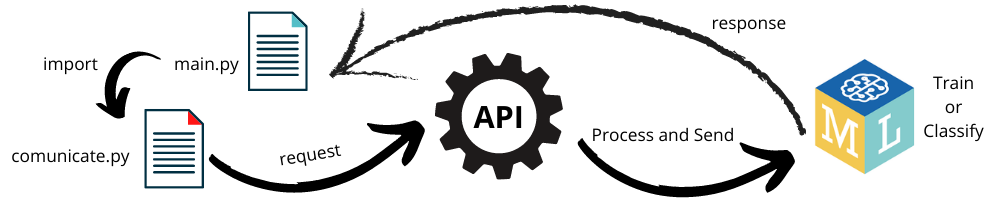
\includegraphics[scale=0.5]{img/api_diagram.png}
\caption{API Diagram}
\label{figure_6}
\end{figure}


\subsection{Training the IA:}
All computer training is performed by Watson, who uses Convolutional Neural Network and linear regression models for classification. Thus, 50 gestures were initially added for each vowel, made by different people, with the right and left hands and on different webcams, to generate greater precision in the results.

\begin{figure}[!ht]
\centering
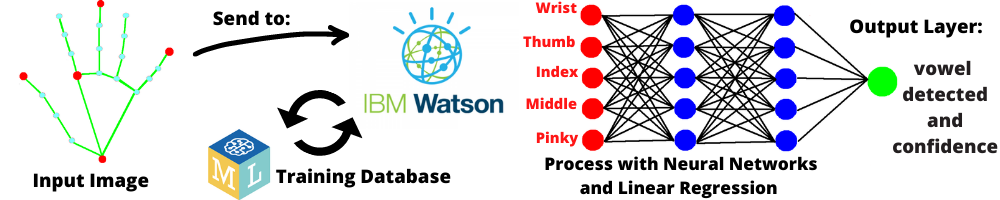
\includegraphics[scale=0.5]{img/training_diagram.png}
\caption{Training Diagram}
\label{figure_7}
\end{figure}

The data entry process for the training database has been automated, now being done by pressing a keyboard key, specific for each vowel gesture.
To facilitate the visualization of the main vertices, it was decided to highlight these points in the webcam window. It was also decided to print in this window a text with the return of the request made.

%%%%%%%%%%%%%%%%%%%%%%%%%%%%%%%%%%%%%%%%%%%%%%%%%%%%%%%%%%%%
\section{Results Analysis}

During the analysis of the results, which took place on 8/21/2021, Machine Learning For Kids had problems to return the confidence percentage, always showing 100\% confidence in all tests performed (correct and wrong). Therefore, to verify the real confidence of this judge, the general average was used, through the number of hits and errors collected for each vowel. So, the following data were collected:


\begin{table}[h!]
    \centering
    \begin{tabular}{ |c|c|c|c|c| } 
    \hline
    \multicolumn{5}{|c|}{Results Analysis - 08/21/2021} \\
    \hline
    Gesture & Tests Done & Corrects & Wrongs & Hit Average \\
    \hline
    A & 20 & 12 & 8 & 60\% \\ 
    \hline
    E & 20 & 15 & 5 & 75\% \\
    \hline
    I & 20 & 18 & 2 & 80\% \\
    \hline
    O & 20 & 12 & 8 & 60\% \\
    \hline
    U & 20 & 17 & 3 & 85\% \\
    \hline
    \end{tabular}
    \caption{Results Analysis}
    \label{tab:results_analysis}
\end{table}

It was noticed that the highest error rate was with vowels A and O, a possible justification is that, graphically, the location of the points is similar. In addition, the errors in the other vowels occurred mainly when the hand was at a distance greater than 1 meter from the webcam. Therefore, 50 more gestures were added to the training database (totaling 100 cases of examples per vowel), and new results were obtained:

\begin{table}[h!]
    \centering
    \begin{tabular}{ |c|c|c|c|c| } 
    \hline
    \multicolumn{5}{|c|}{New Results Analysis - 08/22/2021} \\
    \hline
    Gesture & Tests Done & Corrects & Wrongs & Hit Average \\
    \hline
    A & 30 & 28 & 2 & 93.3\% \\ 
    \hline
    E & 30 & 29 & 1 & 96.6\% \\
    \hline
    I & 30 & 30 & 0 & 100\% \\
    \hline
    O & 30 & 29 & 1 & 96.6\% \\
    \hline
    U & 30 & 30 & 0 & 100\% \\
    \hline
    \end{tabular}
    \caption{New Results Analysis}
    \label{tab:results_analysis2}
\end{table}

With these more accurate results and with a percentage of correct answers above 90\%, it is concluded that this application has high reliability in judging vowels by the Brazilian Sign Language made by hand.

%%%%%%%%%%%%%%%%%%%%%%%%%%%%%%%%%%%%%%%%%%%
\section{Conclusion}

Learning signs using the Brazilian Sign Language will continue to be a challenge not only for hearing impaired people, but also for the entire population. However, applications like this one, which are in the public domain, can serve not only to learn more about the subject, but also to inspire other applications.

The application has already shown itself capable of fulfilling its initial function - recognizing vowels made with manual gestures by LIBRAS -. It uses Machine Learning and, therefore, learns with each interaction, which makes it increasingly intelligent. It can be used in the area of education, both in the use of the application itself, as for teaching, LIBRAS or for teaching subjects related to Machine Learning, it can also be improved by adding another machine learning model, or adding more vertices, even even doing it in another programming language making it more accessible to other audiences.

%%%%%%%%%%%%%%%%%%%%%%%%%%%%%%%%
%  References
\newpage
{\color{white}\section{References}}
\bibliography{ref.bib}
\bibliographystyle{plain}

\end{document}